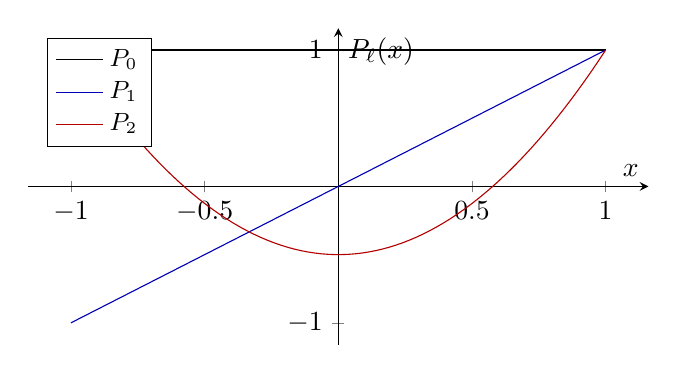
\begin{tikzpicture}
\begin{axis}[
    width=0.78\textwidth,
    height=5.6cm,
    xlabel={$x$},
    ylabel={$P_{\ell}(x)$},
    domain=-1:1,
    samples=80,
    legend pos=north west,
    legend style={font=\small},
    axis lines=middle,
    enlargelimits=0.08,
  ]
  \addplot[black] {1};
  \addplot[blue!70!black] {x};
  \addplot[red!70!black] {0.5*(3*x^2-1)};
  \legend{$P_0$,$P_1$,$P_2$}
\end{axis}
\end{tikzpicture}
